\documentclass[%
 reprint,
%superscriptaddress,
%groupedaddress,
%unsortedaddress,
%runinaddress,
%frontmatterverbose, 
%preprint,
%showpacs,preprintnumbers,
%nofootinbib,
%nobibnotes,
%bibnotes,
 amsmath,amssymb,
 aps,
%pra,
%prb,
%rmp,
%prstab,
%prstper,
%floatfix,
]{revtex4-1}

\usepackage{graphicx}% Include figure files
\usepackage{dcolumn}% Align table columns on decimal point
\usepackage{bm}% bold math
%\usepackage{hyperref}% add hypertext capabilities
%\usepackage[mathlines]{lineno}% Enable numbering of text and display math
%\linenumbers\relax % Commence numbering lines

%\usepackage[showframe,%Uncomment any one of the following lines to test 
%%scale=0.7, marginratio={1:1, 2:3}, ignoreall,% default settings
%%text={7in,10in},centering,
%%margin=1.5in,
%%total={6.5in,8.75in}, top=1.2in, left=0.9in, includefoot,
%%height=10in,a5paper,hmargin={3cm,0.8in},
%]{geometry}

\usepackage{cmap} % Поиск в PDF
\usepackage[T2A]{fontenc} % Кодировка
\usepackage[utf8]{inputenc} % Кодировка исходного текста
\usepackage[english, russian]{babel} % Локализация и переносы
\frenchspacing % Более тонкая настройка пробелов 
\usepackage{multirow}
\usepackage[warn]{mathtext}
\usepackage{amssymb}
\usepackage{ dsfont }

% Переопределение англоязычного начертания каппа, фи и эпсилон, 
% а также знаков сравнения
\renewcommand{\epsilon}{\ensuremath{\varepsilon}}
\renewcommand{\phi}{\ensuremath{\varphi}} 
\renewcommand{\kappa}{\ensuremath{\varkappa}}
\renewcommand{\le}{\ensuremath{\leslant}}
\renewcommand{\leq}{\ensuremath{\leqslant}}
\renewcommand{\ge}{\ensuremath{\geslant}}
\renewcommand{\geq}{\ensuremath{\geqslant}}
\renewcommand{\emptyset}{\ensuremath{\varnothing}}

\usepackage{textcomp} 
\usepackage{indentfirst} % Красная строка
\usepackage{amsmath} % Текст в формулах
\usepackage{graphicx} % Графика
\DeclareGraphicsExtensions{.pdf,.png,.jpg}
\usepackage{pgfplots}
\pgfplotsset{compat=1.13}

%\usepackage{times}

\begin{document}

\title{Диа-~и парамагнетики}
\thanks{3.4.1}

\author{Иван Едигарьев,}
\affiliation{
 Московский Физико-Технический Институт\\
 Факультет Общей и Прикладной Физики, 526т\\
}
%\date{\today}

\begin{abstract}
Цель работы: измерение магнитной восприимчивости диа- и парамагнитного образцов.

В работе используются: электромагнит, аналитические весы, миливеберметр, амперметр постоянного тока, реостаты, образцы.\\

\end{abstract}

\pacs{Valid PACS appear here}% PACS, the Physics and Astronomy
                             % Classification Scheme.
%\keywords{Suggested keywords}%Use showkeys class option if keyword
                              %display desired
\maketitle

%\tableofcontent

\section{\label{sec:level1}Теоретическая справка}

При смещении образца на расстояние $\Delta{l}$ вниз магнитная сила, действующая на него, равна
\begin{equation}\label{1}
    F = \left(\frac{\Delta{W_m}}{\Delta{l}}\right)_I,
\end{equation}
Магнитная энергия рассчитывается по формуле
\begin{equation}\label{2}
    W_m = \frac{1}{2}\int HB dv = \frac{1}{2 \mu_0}\int \frac{B^2}{\mu}dV,
\end{equation} 
Получим для изменения энергии поля:
\begin{equation*}
    \Delta{}W_m = \frac{1-\mu}{2 \mu_0 \mu}B^2s\Delta{l} = -\frac{\chi}{2 \mu_0 \mu}B^2s\Delta{l}.
\end{equation*}

Следовательно, на образец действует сила
\begin{equation}\label{3}
    F = -\frac{\chi}{2 \mu_0 \mu}B^2s.
\end{equation}

Знак силы, действующей на образец, зависит от знака $\chi$: образцы из парамагнитных материалов ($\chi$ > 0) втягиваются в зазор электромагнита, а диамагитные образцы ($\chi$ < 0) выталкиваются из него. 

Пренебрегая отличием $\mu$ от единицы, получаем окончательно рассчётную формулу в виде
\begin{equation}\label{4}
    F = -\frac{\chi B^2s }{2 \mu_0}.
\end{equation}

\begin{center}
    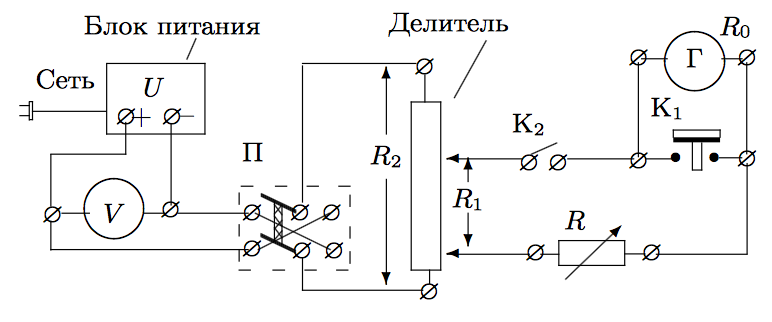
\includegraphics[scale = 0.30]{pic1.png} 
\end{center}



\section{\label{sec:level1}Экспериментальная установка}
Экспериментальная установка. Схема установки изображена на рис. Магнитное поле с максимальной индукцией $\simeq$ 1,5 Тл создаётся в зазоре электромагнита, питаемого постоянным током. Диаметр полюсов существенно превосходит ширину зазора, поэтому поле в средней части зазора достаточно однородно. Величина тока, проходящего через обмотки электромагнита, регулируется при помощи трёх реостатов $R_1$, $R_2$ и $R_3$ и измеряется многопредельным амперметром А. Тонкая проволока высокоомных реостатов не рассчитана на большой ток, поэтому регулировку более низкоомными реостатами следует проводить только при полностью выведенных высокоомных реостатах.

Градуировка электромагнита (связь между индукцией магнитного поля $В$ в зазоре электромагнита и силой тока $I$ в его обмотках) производится при помощи милливеберметра.

При измерениях образцы поочерёдно подвешиваются к аналитическим весам так, что один конец образца оказывается в зазоре электромагнита, а другой — вне зазора, где индукцией магнитного поля можно пренебречь. При помощи аналитических весов определяется перегрузка $\Delta{P} = F$ - сила, действующая на образец со стороны магнитного поля.

Как уже отмечалось, силы, действующие на диа- и парамагнитные образцы, очень малы. Небольшие примеси ферромагнетиков (сотые доли процента железа или никеля) способны кардинально изменить результат опыта, поэтому образцы были специально отобраны.

\section{\label{sec:level1}Задание}

В работе предлагается исследовать зависимость силы, действующей на образец, размещённый в зазоре электромагнита, от величины поля в зазоре и по результатам измерений рассчитать магнитную восприимчивость меди и алюминия.\\
1. Проверьте работу цепи электромагнита. Оцените диапазон изменения тока $I$ через обмотки.\\
2. Прокалибруйте электромагнит. Для этого с помощью милливеберметра снимите зависимость магнитного потока $\Phi$, пронизывающего пробную катушку, находящуюся в зазоре, от тока $I$ ($\Phi = BSN$). Значение $SN$ (произведение площади сечения пробной катушки на число витков в ней) указано на установке.

\begin{center}
    \textbf{Включать и отключать электромагнит следует только при минимальном токе.}
\end{center}
3.	Убедитесь, что весы арретированы.
\begin{center}
    \textbf{Весы следует арретировать перед каждым изменением тока.}
\end{center}
4.	Измерьте силы, действующие на образец в магнитном поле. Для этого, не включая электромагнит, подвесьте к весам один из образцов. Установите на весах примерное значение массы образца (масса, диаметр и максимальное значение перегрузки для каждого образца указаны на установке). Освободите весы и добейтесь точного равновесия весов.

Арретируйте весы. Установите минимальное значение тока и проведите измерение равновесного значения массы.

Повторите измерения $m = f(T)$ для 6-8 других значений тока.\\
5.	Повторите измерения п. 4 для другого образца.

\begin{center}
Обработка результатов
\end{center}
1. Рассчитайте поле $B$ и постройте градуировочную кривую для электромагнита: $B = f(I)$.\\
2. Постройте на одном листе графики |$\Delta{P}$| = $f(B^2)$ для меди и алюминия.\\
3. По наклонам полученных прямых рассчитайте величину $\chi$ с помощью формулы (4).\\
4. Оцените погрешности измерений и сравните результаты с табличными значениями.

\section{\label{sec:level1}Данные.}

Посмотрим на данные калибровки электромагнита. При проведении эксперимента была исследована зависимость $I(\Phi)$ при увеличении и уменьшении тока. Построим на одном графике данные измерения.

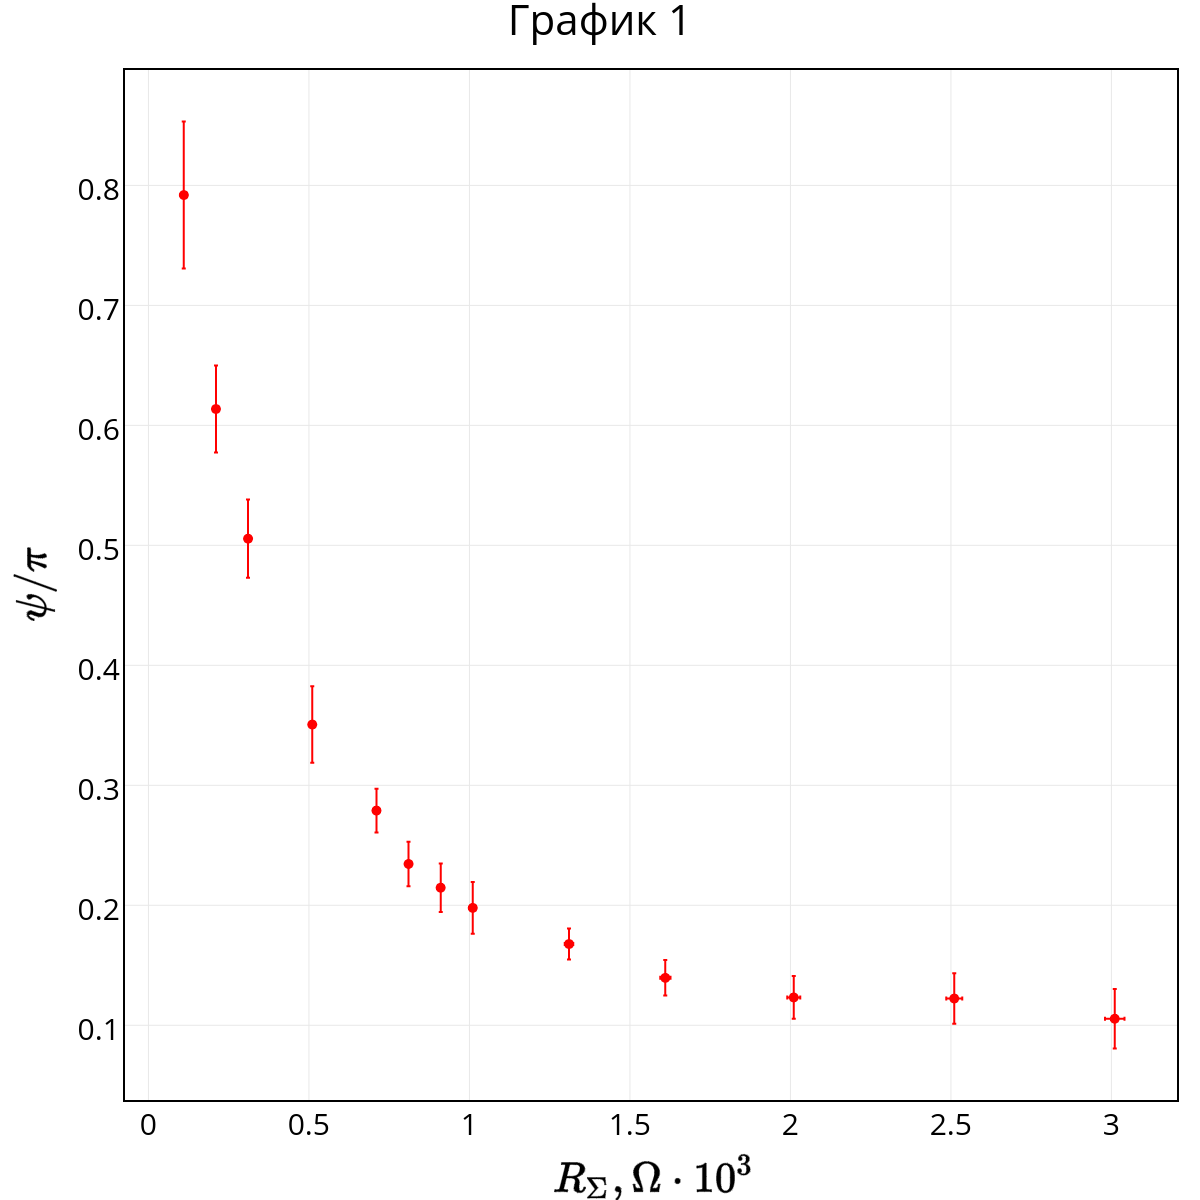
\includegraphics[scale = 0.19]{my_plot1.png}

Как можно видеть влиянием эффекта гистерезиса можно пренебречь. Для дальнейшего анализа усредним значения по двум наборам и пренебрежём статистической ошибкой $\Phi$. Зафиксируем значение систематической ошибки измерения $\Phi$ и перейдём к значениям магнитного поля $B$.

Во время проведения эксперимента было измерена зависимость силы $F$, выраженной с точностью до умножения на известный множитель в $\Delta{m}$, от значения тока в обмотках электромагнита $I$ для двух материалов, алюминия и меди соответственно. Обе зависимости состояли из 11 серий при увеличении тока, в каждой серии было проведено 3 измерения. 

Усредним значение $\Delta{m}$ в каждой серии и вычислим оценочную дисперсию $\Delta{m}$ для каждого значения тока $I$. Построим на одном графике зависимость $|\Delta{m}|$ от $B^2$ для обоих материалов.

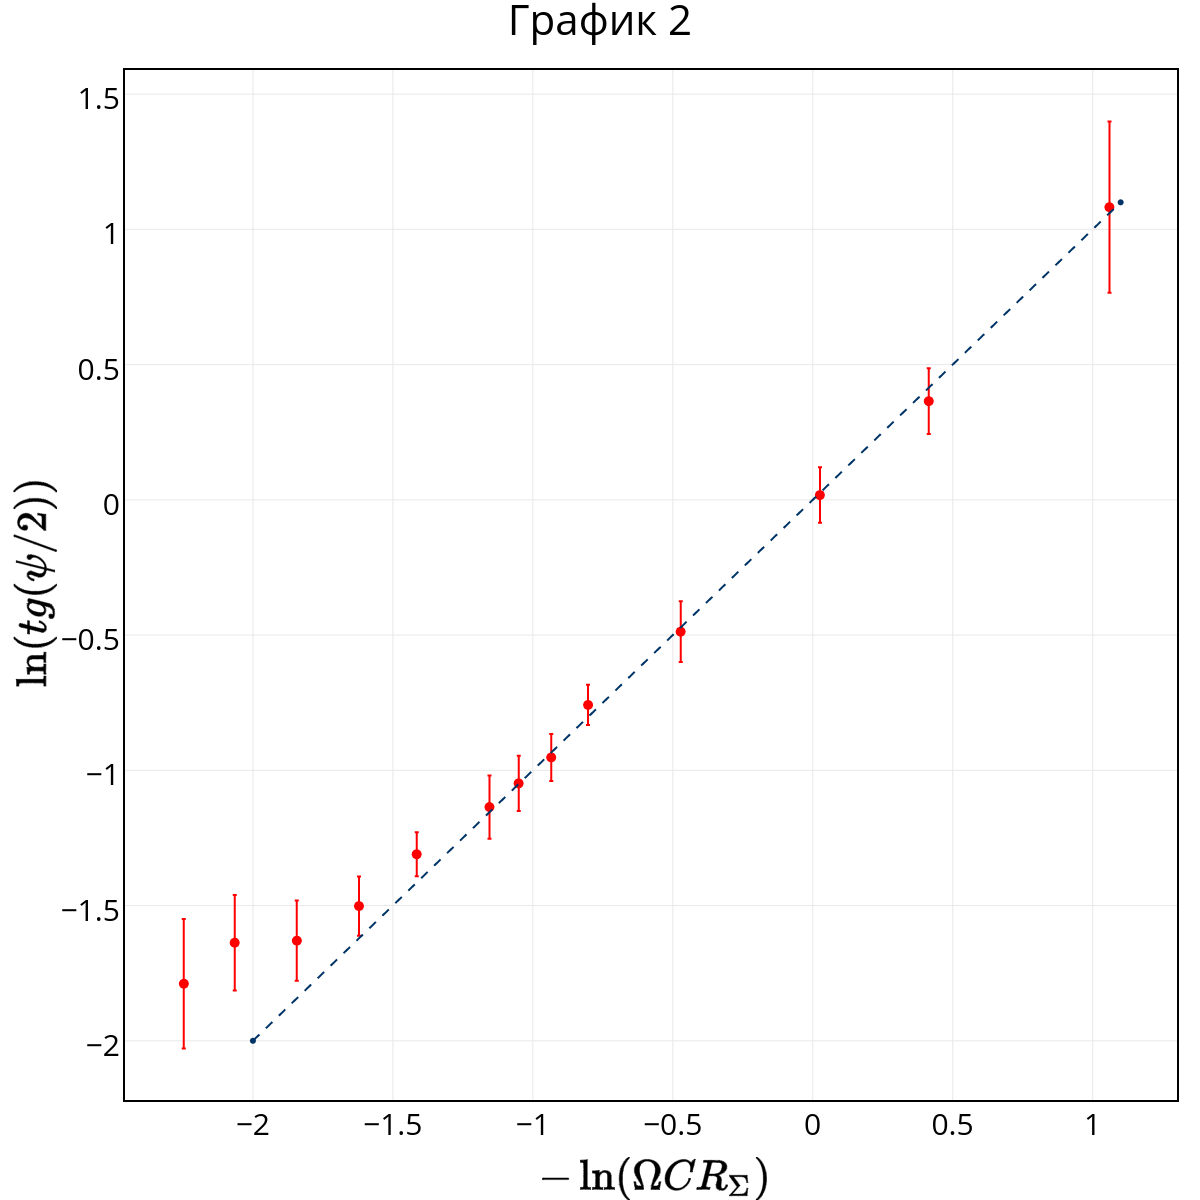
\includegraphics[scale = 0.19]{my_plot2.png} 

Легко видеть, что линейность обоих зависимостей выражена. Построим простой метод наименьших квадратов (least squares) для обоих образцов:
$$ \alpha, \beta = \text{argmin}_{\beta}(\sum_i^n (y_i - \alpha - \beta x_i)^2) $$

Вычислим статистические ошибки параметров модели и построим график зависимости отклика для каждого измерения $\Delta{m}$ от $B^2$, а также 95\% доверительный интервал для этого отклика:\\
\\
Cu:

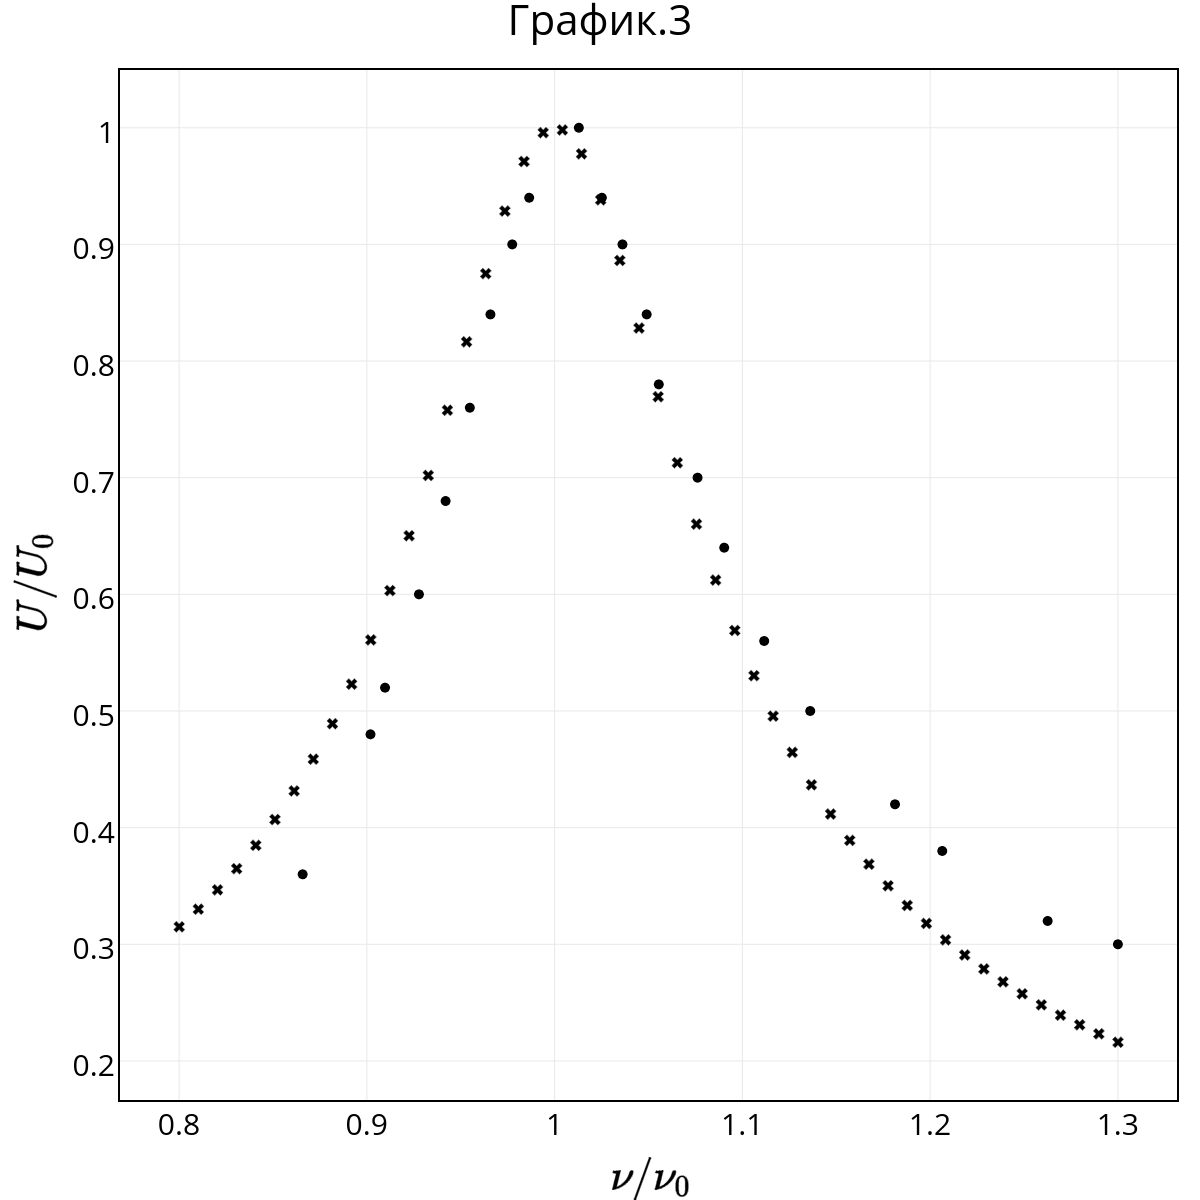
\includegraphics[scale = 0.19]{my_plot3.png}\\
\\
Al:

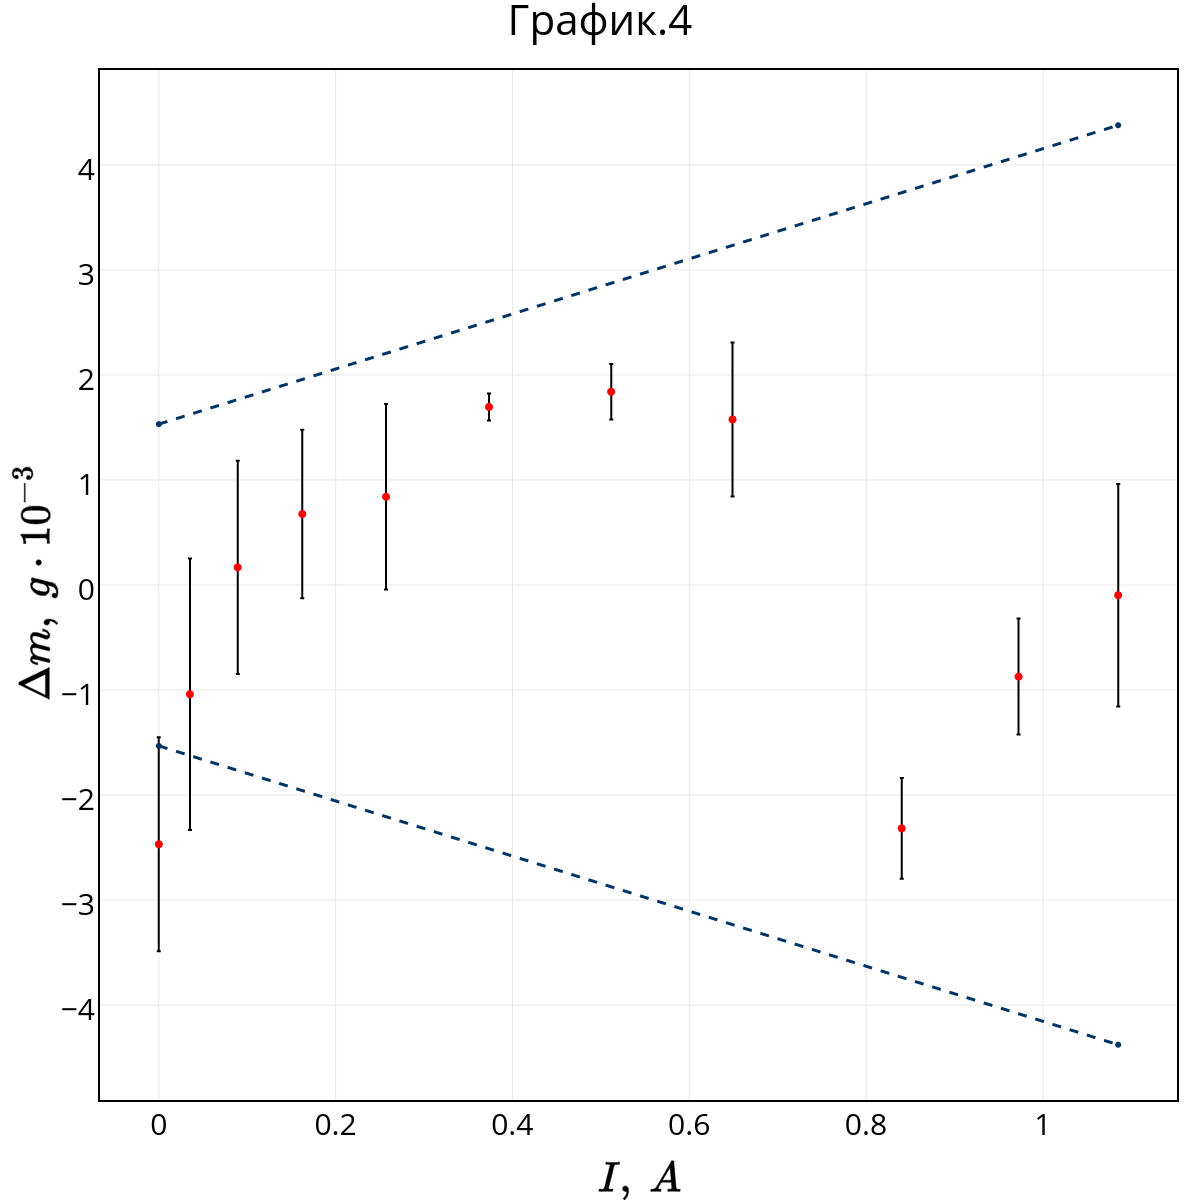
\includegraphics[scale = 0.19]{my_plot4.png} 
\newpage

Видим, что обе модели согласуются с измеренными данными c точностью до 95\% доверительного интервала. Итоговые параметры:

$$ \alpha_{\text{Cu}} = (7 \pm 3) \times 10^{-4}~\text{g},~~\beta_{\text{Cu}} = (220 \pm 5^{\text{stat}}) \times 10^{-4}~\text{g/T}$$
$$ \alpha_{\text{Al}} = (24 \pm 7) \times 10^{-4}~\text{g},~~\beta_{\text{Al}} = (665 \pm 13^{\text{stat}}) \times 10^{-4}~\text{g/T}$$

Теперь вычислим значения $\chi$ для обоих материалов, оценим статистическую и систематическую ошибку:

$$\chi_{\text{Cu}} = (-70 \pm 10^{\text{stat}} \pm 5^{syst}) \times 10^{-7}$$
$$\chi_{\text{Al}} = (213 \pm 30^{\text{stat}} \pm 16^{syst}) \times 10^{-7}$$


Табличные значения для материалов:

$$\chi^{\text{std}}_{\text{Cu}} = -103 \times 10^{-7}$$
$$\chi^{\text{std}}_{\text{Al}} = 230 \times 10^{-7}$$


\end{document}

